% Short (5-page) course report in the NeurIPS 2026 format.
% In Overleaf: open the "Formatting Instructions for NeurIPS 2026" template, replace its main .tex with
% this file and upload the figures/ folder. neurips_2026.sty comes with that template.
% Without the style file (local preview), a close stand-in layout is used instead.
\documentclass{article}

\PassOptionsToPackage{numbers, compress}{natbib}
\IfFileExists{neurips_2026.sty}{%
  \usepackage[preprint]{neurips_2026}%
}{%
  \usepackage[letterpaper, textwidth=5.5in, textheight=9in, top=1in, headheight=12pt, headsep=25pt, footskip=30pt]{geometry}%
  \usepackage{times}%
  \usepackage{natbib}%
  \AtBeginDocument{\def\And{\quad}\def\AND{\\}}%
}

\usepackage[utf8]{inputenc}
\usepackage[T1]{fontenc}
\usepackage{hyperref}
\usepackage{url}
\usepackage{booktabs}
\usepackage{amsmath}
\usepackage{amsfonts}
\usepackage{nicefrac}
\usepackage{microtype}
\usepackage{xcolor}
\usepackage{graphicx}
\usepackage[font=small, labelfont=bf, skip=3pt]{caption}

\newcommand{\tms}{\ensuremath{\times}}

\title{How Far to Guess? Testing Hardware-Aware Draft Sizes for Speculative Decoding on Everyday Devices and Indian Languages}

\author{%
  Pranjal Kirar (230106050) \And Aditya Raj (230121004) \And Khushal Nagwal (230106035) \AND
  Babita Verma (230106015) \And Yash Pratap Singh (230106084) \\[4pt]
  DA4022 Hardware-Aware Deep Learning, Project 22
}

\begin{document}

\maketitle

\begin{abstract}
Speculative decoding makes a language model write faster by guessing several tokens ahead and checking them all in one pass.
Two recent papers, UniSpec and PPD, choose how many tokens to guess with the same rule: pick the draft size $g$ that maximises tokens gained per pass divided by the time of a pass.
Both papers tested this rule on large data-centre GPUs.
We test it on a laptop CPU, two laptop GPUs (Apple M1 and RTX 3060) and a free cloud GPU (Tesla T4), with a small model and news summaries in English, Hindi, Marathi, Bengali and Tamil.
The number of accepted tokens was the same on every device (within 0.07 tokens), so this part of the rule holds.
The time of a pass was not: on the CPU, checking 33 tokens took 3.8 times as long as one token, while on the T4 it took only 1.2 times as long.
As a result the CPU and the M1 were fastest with 8 guessed tokens (1.53\tms{} and 1.71\tms{}), while the two NVIDIA GPUs stayed flat at about 2.1--2.3\tms{} for any size from 12 upwards.
Using a GPU's draft size on the CPU cost 8--17\% of the speed.
UniSpec's curve fit found the best size on the CPU and the M1 but over-predicted the speedup on the NVIDIA GPUs by 25--31\%.
Indian languages were accepted far more often than English, but their long prompts made reading the input the main cost on the CPU.
\end{abstract}

\section{Introduction}

Large language models (LLMs) produce text one token at a time.
Each new token needs a full pass through the network, and that pass is mostly spent reading the model's weights from memory.
On a GPU this means that a pass over ten tokens costs about the same as a pass over one.
Speculative decoding uses this spare capacity~\citep{leviathan, chen}.
A cheap \emph{drafter} guesses the next $g$ tokens, and the model checks all of them in one pass.
We keep every guessed token the model agrees with and stop at the first one it rejects.
With greedy decoding the output is exactly the same as normal decoding; only the time changes.

The draft size $g$ is a trade-off.
More guesses can give more accepted tokens per pass, but a longer pass also takes more time.
UniSpec~\citep{unispec} and PPD~\citep{ppd} both choose $g$ with the same rule:
\begin{equation}
  \text{speedup}(g) \;=\; \frac{\tau(g)}{s(g)},
  \label{eq:rule}
\end{equation}
where $\tau(g)$ is the average number of tokens gained per pass and $s(g)$ is the time of one pass with $g$ guesses, relative to a normal pass.
The idea is that $\tau$ depends only on the model and the text, while $s$ depends only on the hardware.
So $\tau$ could be measured once, and only $s$ would need timing on each new device.
Both papers tested this on data-centre and high-end desktop GPUs.

We ask whether the rule still holds on hardware that students and small teams actually have, and in Indian languages, which the papers did not test.
Our four questions are:
(1) Is $\tau$ really the same on every device?
(2) How different is $s(g)$, and does the best $g$ change?
(3) How much speed is lost with a draft size tuned on another device?
(4) Do UniSpec's and PPD's ways of choosing $g$ work there, and what changes for Indian languages?

\section{Background}

\textbf{Drafters.}
A drafter can be a small separate model~\citep{leviathan}, extra prediction heads trained on the main model~\citep{medusa, eagle}, or something with no training at all.
We use the simplest training-free option, an \emph{n-gram} or prompt-lookup drafter~\citep{pld}.
It looks for the last few written tokens earlier in the text (including the prompt) and proposes what followed them there.
It costs almost nothing to run, which keeps the comparison focused on the main model.

\textbf{UniSpec}~\citep{unispec} is a training-free method that also uses n-gram drafting.
Its \emph{device-aware calibration} runs the model on a few calibration examples, fits a saturating curve to $\tau(g)$ and a quadratic curve to the pass time, and picks the $g$ that maximises their ratio.

\textbf{PPD}~\citep{ppd} trains special prompt tokens to draft.
For choosing $g$ it splits Equation~\ref{eq:rule} in two: $\tau(g)$ is measured once on any device, and $s(g)$ comes from a short timing profile of the target device, read at the average number of tokens per pass.
Training PPD's tokens takes about 16 GPU hours on an A100, which we could not afford, so we use only its way of choosing $g$, with our n-gram drafter.

\section{Experimental setup}

\textbf{Model, task and data.}
We use Qwen2.5-0.5B-Instruct~\citep{qwen}, small enough for any laptop.
The task is summarising BBC news articles from XL-Sum~\citep{xlsum} in 4--5 sentences, cut to the first 250 words.
We use English, Hindi, Marathi, Bengali and Tamil.
Decoding is greedy with 128 new tokens.
Half of the English articles are used to choose $g$ (\emph{calibration}) and the other half to check that choice (\emph{held-out}).

\textbf{Devices.}
Table~\ref{tab:devices} lists the four devices.
The CPU uses 32-bit numbers; all GPUs use 16-bit numbers.
The same command runs on every device and detects the hardware itself.
We ran a second, wider sweep on the T4 with $g$ up to 128.

\begin{table}[t]
\centering
\small
\caption{Devices. Pass time is one pass over one new token at a 1,024-token context. ``Cost of 33'' is a pass over 33 tokens relative to that.}
\label{tab:devices}
\begin{tabular}{llrrc}
\toprule
Device & Type & 1-token pass & Cost of 33 & Articles (calib + held-out) \\
\midrule
Intel Core i7-8550U & laptop CPU, fp32 & 130 ms & 3.80\tms & 6 + 6 \\
Apple M1 (MacBook Air) & integrated laptop GPU, fp16 & 33 ms & 2.81\tms & 6 + 6 \\
NVIDIA RTX 3060 Laptop & gaming laptop GPU, fp16 & 53 ms & 1.07\tms & 6 + 6 \\
NVIDIA Tesla T4 (Colab) & free cloud GPU, fp16 & 24 ms & 1.23\tms & 15 + 15 \\
\bottomrule
\end{tabular}
\end{table}

\textbf{Engine and checks.}
We wrote a small decoding loop in PyTorch~\citep{pytorch} and Hugging Face Transformers~\citep{transformers}.
Normal decoding and speculative decoding run through the same loop, so their timings are comparable.
After each pass we remove the rejected guesses from the model's cache.
We first check that speculative output is identical to normal output.
It was identical on the CPU every time.
On the GPUs a few runs (up to 17\% on the M1, 10\% on the T4 and 8\% on the RTX 3060 at a given $g$) changed after a near-tie between two tokens, a known rounding effect of 16-bit numbers.

\textbf{Experiments.}
(i) A \emph{hardware profile} times passes over 1 to 33 new tokens (129 on the T4).
(ii) A \emph{sweep} decodes each article normally and then with $g$ = 1, 2, 3, 4, 6, 8, 12, 16, 24 and 32, back to back.
(iii) \emph{Calibration} chooses $g$ from the calibration articles in three ways: grid search, UniSpec's curve fit, and PPD's split, and then measures the choice on the held-out articles.
(iv) A \emph{language study} runs five or more articles per language.
(v) A \emph{load test} runs the CPU and the M1 non-stop for 20 minutes.

\textbf{How we average.}
We report speedup as total time of normal decoding divided by total time of speculative decoding over all articles.
An early version averaged each article's own speedup instead.
One T4 article whose summary copied its source almost word for word ran 39.8\tms{} faster and pulled that average up to 4.10\tms{}, while the total-time speedup was 2.20\tms.
Averages of ratios are easily dominated by one unusual article.

\section{Results}

\subsection{Acceptance is the same on every device}

On the 12 articles that every device summarised, $\tau$ agreed within 0.07 at every draft size (Figure~\ref{fig:sweep}, left).
For example, $\tau$ was 2.18 on the CPU, the M1 and the T4 at $g$ = 8.
The small differences come from the 16-bit near-ties above.
So the shared assumption of UniSpec and PPD holds on our devices: acceptance can be measured once.

\begin{figure}[t]
\centering
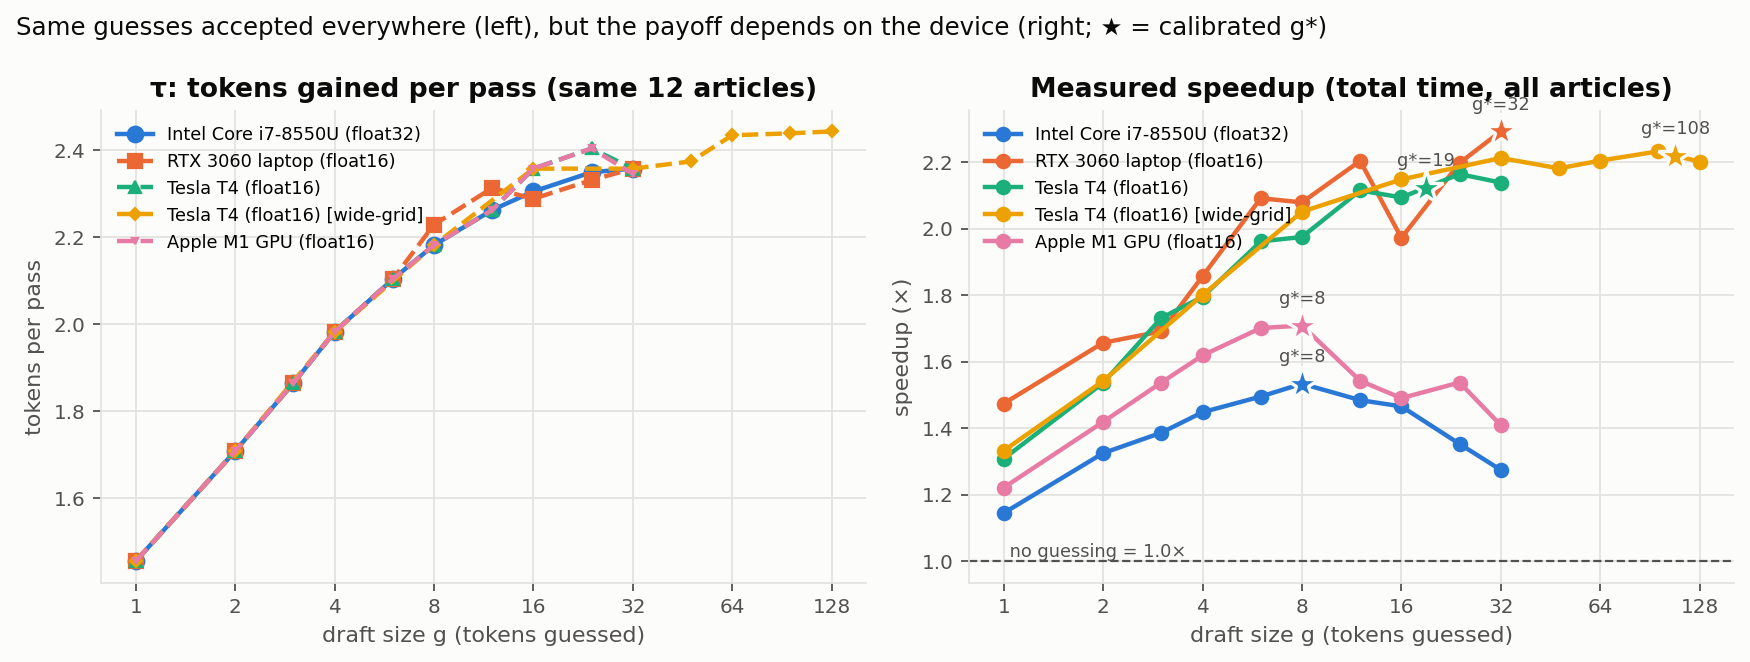
\includegraphics[width=\linewidth]{figures/fig2_draft_size_sweep.png}
\caption{Left: tokens gained per pass on the 12 articles run on every device; the lines lie on top of each other. Right: measured speedup (total time) by draft size. Stars mark the size chosen by UniSpec's fit.}
\label{fig:sweep}
\end{figure}

\subsection{The cost of a pass is not, so the best draft size differs}

The devices charge very differently for extra tokens (Table~\ref{tab:devices}).
On the CPU, a pass over two tokens already costs 1.54\tms{} a one-token pass, and 33 tokens cost 3.80\tms.
On the T4, 33 tokens cost only 1.23\tms, and even 129 tokens take just 36.9 ms.
The M1 is in between (2.81\tms{} for 33 tokens).
The RTX 3060 is flat like the T4 (1.07\tms), but its passes are slow for a GPU, about 50--60 ms, and changed from 52 to 73 ms between articles.
That points to a fixed cost per pass on that Windows laptop rather than to the GPU itself.

Because $\tau$ is shared and the pass time is not, the speedup curves differ (Figure~\ref{fig:sweep}, right).
The CPU is fastest at $g$ = 8 (1.53\tms) and drops to 1.27\tms{} at $g$ = 32, where 4 of its 12 articles were slower than normal decoding.
The M1 behaves like the CPU, not like the other GPUs: 1.71\tms{} at $g$ = 8 and 1.41\tms{} at $g$ = 32.
So being a GPU is not enough; what matters is how fast the pass time grows.
The T4 reaches 2.11\tms{} at $g$ = 12 and then stays flat up to $g$ = 128 (2.20\tms).
The RTX 3060 also stays high, with its best tested value of 2.29\tms{} at $g$ = 32, but its curve is bumpy because of its noisy timings.
On the GPUs larger drafts cost almost nothing, but they also gain almost nothing, because $\tau$ stops growing at about 2.4 tokens for English.

\subsection{A draft size from another device costs speed on the CPU and the M1}

Table~\ref{tab:calib} (right column) and the held-out articles show what happens with the ``wrong'' $g$.
The CPU loses 8\% with the T4's calibrated size ($g$ = 19) and 17\% with the largest size ($g$ = 32).
The M1 loses 13\% and 19\%.
The T4 loses only 4--5\% with the CPU's $g$ = 8.
On the RTX 3060, sizes from 8 to 32 gave 1.79--2.02\tms{} against 1.99\tms{} with its own choice, which is within its timing noise.
No device fell below 1.0\tms{} overall, but single articles did on the CPU and the M1.
So a wrong setting mainly hurts devices that pay for every extra token.

\subsection{Choosing the draft size automatically}

\begin{table}[t]
\centering
\small
\caption{Draft size chosen on the calibration articles and its result on the held-out articles. Predicted and measured are generation-only speedups; end to end includes reading the prompt.}
\label{tab:calib}
\begin{tabular}{llrrrr}
\toprule
Device & Method & $g$ & Predicted & Measured & End to end \\
\midrule
Intel i7 CPU & Grid search & 8 & 1.68\tms & 1.68\tms & 1.53\tms \\
             & UniSpec fit & 8 & 1.70\tms & 1.68\tms & 1.53\tms \\
             & PPD split   & 9 & 1.41\tms & 1.66\tms & 1.51\tms \\
\midrule
Apple M1     & Grid search & 6 & 1.80\tms & 1.75\tms & 1.67\tms \\
             & UniSpec fit & 8 & 1.76\tms & 1.78\tms & 1.69\tms \\
             & PPD split   & 12 & 1.89\tms & 1.56\tms & 1.51\tms \\
\midrule
RTX 3060     & Grid search & 12 & 2.67\tms & 1.85\tms & 1.83\tms \\
             & UniSpec fit & 32 & 2.66\tms & 2.03\tms & 1.99\tms \\
             & PPD split   & 27 & 2.88\tms & 1.95\tms & 1.92\tms \\
\midrule
Tesla T4     & Grid search & 24 & 2.47\tms & 1.94\tms & 1.92\tms \\
             & UniSpec fit & 19 & 2.41\tms & 1.92\tms & 1.91\tms \\
             & PPD split   & 16 & 2.29\tms & 1.91\tms & 1.90\tms \\
\bottomrule
\end{tabular}
\end{table}

On the CPU, UniSpec's fit and grid search both chose $g$ = 8, the best size tested, and the fit predicted 1.70\tms{} against 1.68\tms{} measured (Table~\ref{tab:calib}).
On the M1 the fit again chose 8 and was just as close (1.76\tms{} against 1.78\tms).
PPD's split chose $g$ = 12 there and was 12\% slower.
It reads the pass time at the \emph{average} pass, about five tokens, and so misses the jump in cost the M1 shows between 9 and 13 tokens.
Taking $\tau$ from another device changed PPD's choice by at most one.

On both NVIDIA GPUs every method landed close together, because their curves are flat.
But the fit over-predicted by 25--31\%.
On their own calibration articles the fitted curves were within 4\% of the measurements on every device, so the fit itself works.
The problem was that the held-out articles behaved differently.
On the T4 the calibration articles were easier: their summaries copied 60\% of their 4-token pieces from the article against 43\% for the held-out ones, and $\tau$ at $g$ = 32 was 2.75 against 2.07.
On the RTX 3060 the articles were alike, but the timings drifted: a normal pass took 62.8 ms on the calibration half and 57.7 ms on the held-out half.
Calibration is only as good as how typical its inputs are.

\subsection{The text matters as much as the hardware}

Across articles, speedup closely followed how much the summary copied from the article (correlation 0.78--0.87 across devices).
On the CPU, an English summary that copied about 20\% ran 1.1\tms{} faster; one that copied 91\% ran 3.4\tms{} faster.
The hardware decides how far it is worth guessing; the text decides how much there is to gain.

\subsection{Indian languages}

Qwen2.5's tokenizer splits English into 1.3 tokens per word, but Hindi into 4.7, Marathi 6.6, Bengali 7.0 and Tamil 10.1.
The tokenizer of Sarvam-1, a model built for Indian languages, needs only 1.4--2.3 for the same text, so this is a property of the tokenizer, not the languages.
A 250-word Tamil article becomes a prompt about seven times longer than the English one.

We expected more pieces per word to make guessing harder.
The opposite happened (Table~\ref{tab:lang}).
The small model mostly copied the article: 92--100\% of the 4-token pieces in its Indian-language summaries came from the article, against about half in English.
And each copied word is many tokens, so one correct guess gives many tokens at once.
On the GPUs this turned into large gains.
On the CPU it did not: generation alone was 2.7--3.7\tms{} faster, but the whole request only 1.4--1.9\tms{}, because just reading the 2,570-token Tamil prompt took 20 seconds, half of the request.
Guessing cannot speed up reading the prompt.
The RTX 3060 numbers come from only five articles per language and $g$ = 32, so they are less reliable than the T4's twenty.

\begin{table}[t]
\centering
\small
\caption{Whole-request speedup by language, each device at its own draft size. The last column is the time normal decoding spends reading the Tamil prompt.}
\label{tab:lang}
\begin{tabular}{lcccccccc}
\toprule
Device ($g$) & English & Hindi & Marathi & Bengali & Tamil & Tamil read time \\
\midrule
Intel i7 CPU (14) & 1.60\tms & 1.88\tms & 1.63\tms & 1.67\tms & 1.41\tms & 20.1 s \\
Apple M1 (8)      & 1.85\tms & 2.36\tms & 2.15\tms & 2.04\tms & 1.74\tms & 1.5 s \\
RTX 3060 (32)     & 2.43\tms & 9.60\tms & 4.95\tms & 8.99\tms & 6.20\tms & 0.7 s \\
Tesla T4 (32)     & 1.84\tms & 6.53\tms & 5.88\tms & 6.49\tms & 5.23\tms & 0.15 s \\
\bottomrule
\end{tabular}
\end{table}

\subsection{Sustained load}

UniSpec assumes the hardware stays the same over time.
Over 20 minutes of non-stop work the CPU kept a speedup of 1.45--1.51\tms{} and the fanless M1 1.74--1.75\tms{}, with no downward trend.
Neither started cool, so slowing down earlier cannot be ruled out.
In one informal run on battery, a normal CPU pass took about 47\% longer than plugged in.

\section{Discussion and limitations}

The rule in Equation~\ref{eq:rule} holds in the sense the papers rely on: $\tau$ can be measured once and reused.
But the practical answer depends on the shape of $s(g)$.
On devices where every extra token costs time (our CPU and the M1), the draft size matters, a GPU's setting ($g$ = 19 or 32) loses 8--19\% of the speed, and calibration is worth doing.
On GPUs with spare capacity the curve is flat, and almost any size above 12 is fine.

Our study has clear limits.
The model is small (0.5B parameters), while the papers used models from 1.4B to 14B, so a pass is cheap and the GPUs are far from busy.
We use one chain of guesses, not UniSpec's tree of guesses, and we did not train PPD's drafter.
The sweeps on the laptops use only 12 English articles and one run each, and laptop timings are noisy; differences under about 5\% should not be over-read.
Finally, the small model copies heavily in Indian languages; a larger model that paraphrases more would likely accept fewer guesses.

\section{Conclusion}

Acceptance of guessed tokens did not depend on the device, but the cost of checking them did, by a factor of three between a laptop CPU and a cloud GPU.
On the CPU and the M1 the best draft size was 8 and a GPU's setting cost 8--19\%; on the T4 and the RTX 3060 the curve was flat.
UniSpec's calibration found the best size where it mattered, as long as its calibration articles and timings were typical.
For Indian languages, guessing helped much more than for English, but on a laptop the long prompts, caused by the tokenizer, took most of the time.
Our code runs every experiment with one command, so further devices can be added easily.

{\small
\begin{thebibliography}{99}
\bibitem{unispec} D.-T. Do, N.-K. Le, and N. L. Minh. UniSpec: Training-free speculative decoding for robust LLM acceleration across languages and hardware. In \emph{Proceedings of ACL}, pages 6288--6310, 2026.
\bibitem{ppd} H. Chen, W. Luk, K. F. C. Yiu, R. Li, K. Mishchenko, S. I. Venieris, and H. Fan. Hardware-aware parallel prompt decoding for memory-efficient acceleration of LLM inference. In \emph{Findings of EMNLP}, pages 2221--2238, 2025.
\bibitem{leviathan} Y. Leviathan, M. Kalman, and Y. Matias. Fast inference from transformers via speculative decoding. In \emph{Proceedings of ICML}, 2023.
\bibitem{chen} C. Chen, S. Borgeaud, G. Irving, J.-B. Lespiau, L. Sifre, and J. Jumper. Accelerating large language model decoding with speculative sampling. arXiv:2302.01318, 2023.
\bibitem{medusa} T. Cai, Y. Li, Z. Geng, H. Peng, J. D. Lee, D. Chen, and T. Dao. Medusa: Simple LLM inference acceleration framework with multiple decoding heads. In \emph{Proceedings of ICML}, 2024.
\bibitem{eagle} Y. Li, F. Wei, C. Zhang, and H. Zhang. EAGLE: Speculative sampling requires rethinking feature uncertainty. In \emph{Proceedings of ICML}, 2024.
\bibitem{pld} A. Saxena. Prompt lookup decoding. \url{https://github.com/apoorvumang/prompt-lookup-decoding}, 2023.
\bibitem{qwen} Qwen Team. Qwen2.5 technical report. arXiv:2412.15115, 2024.
\bibitem{xlsum} T. Hasan, A. Bhattacharjee, M. S. Islam, K. Mubasshir, Y.-F. Li, Y.-B. Kang, M. S. Rahman, and R. Shahriyar. XL-Sum: Large-scale multilingual abstractive summarization for 44 languages. In \emph{Findings of ACL-IJCNLP}, 2021.
\bibitem{transformers} T. Wolf et al. Transformers: State-of-the-art natural language processing. In \emph{Proceedings of EMNLP: System Demonstrations}, 2020.
\bibitem{pytorch} A. Paszke et al. PyTorch: An imperative style, high-performance deep learning library. In \emph{Advances in NeurIPS}, 2019.
\end{thebibliography}
}

\end{document}
